% ============================================================
% Práctica Experimental U3 -- Clúster CockroachDB TiendaTech
% Grupo C
% ============================================================
% NOTA: se usa article + twocolumn en vez de IEEEtran.cls porque
% ese paquete no está garantizado en todas las instalaciones. Si
% en tu entorno (Overleaf o TeX Live "completo") tienes
% texlive-publishers instalado, puedes sustituir la siguiente
% línea por: \documentclass[10pt,letterpaper]{IEEEtran}
% sin modificar el resto del documento.
\documentclass[10pt,letterpaper]{article}
\usepackage[twocolumn]{geometry}
\geometry{letterpaper,margin=1.9cm,columnsep=0.6cm}

\usepackage[utf8]{inputenc}
\usepackage[T1]{fontenc}
\usepackage{amsmath,amssymb,amsfonts}
\usepackage{graphicx}
\usepackage{booktabs}
\usepackage{tabularx}
\usepackage{multirow}
\usepackage{xcolor}
\usepackage{listings}
\usepackage{tikz}
\usetikzlibrary{positioning,arrows.meta,calc,shapes.multipart}
\usepackage{hyperref}
\usepackage{caption}
\usepackage{float}
\usepackage{enumitem}
\usepackage{titlesec}
\usepackage{abstract}
\usepackage[numbers,sort&compress]{natbib}
\hypersetup{colorlinks=true,linkcolor=blue,citecolor=blue,urlcolor=blue}

\titleformat{\section}{\normalfont\large\bfseries}{\thesection.}{0.5em}{}
\titleformat{\subsection}{\normalfont\normalsize\bfseries}{\thesubsection}{0.5em}{}
\renewcommand{\refname}{Referencias}
\renewcommand{\abstractname}{Resumen}
\sloppy
\tolerance=2500
\emergencystretch=2.5em
\hbadness=6000
\vbadness=6000

\definecolor{codebg}{RGB}{245,245,245}
\definecolor{codekw}{RGB}{0,0,180}
\definecolor{codecom}{RGB}{95,130,95}
\definecolor{codestr}{RGB}{160,20,20}
\lstdefinestyle{code}{
  backgroundcolor=\color{codebg}, basicstyle=\ttfamily\scriptsize,
  keywordstyle=\color{codekw}\bfseries, commentstyle=\color{codecom}\itshape,
  stringstyle=\color{codestr}, numbers=left, numberstyle=\tiny\color{gray},
  numbersep=6pt, breaklines=true, breakatwhitespace=false, frame=single,
  captionpos=b, tabsize=2, showstringspaces=false
}
\lstdefinelanguage{SQLext}{
  morekeywords={CREATE,TABLE,DATABASE,IF,NOT,EXISTS,USE,PRIMARY,KEY,FOREIGN,
    REFERENCES,CONSTRAINT,CHECK,UNIQUE,DEFAULT,GENERATED,BY,AS,IDENTITY,ALTER,
    PARTITION,LIST,RANGE,VALUES,IN,FROM,TO,MINVALUE,MAXVALUE,SELECT,WHERE,JOIN,
    ON,GROUP,ORDER,LIMIT,EXPLAIN,ANALYZE,COUNT,SUM,AVG,AND,BETWEEN,INTERVAL,DESC,
    SHOW,RANGES,PARTITIONS,TABLES},
  sensitive=false, morecomment=[l]{--}, morestring=[b]'
}
\lstset{style=code}

\begin{document}

%------------------------------------------------------------
% PORTADA
%------------------------------------------------------------
\begin{titlepage}
\begin{center}
{\large \textbf{UNIVERSIDAD TÉCNICA ESTATAL DE QUEVEDO}}\\[2pt]
{\normalsize \textit{La primera universidad agropecuaria del Ecuador}}\\[4pt]
{\large FACULTAD DE CIENCIAS DE LA COMPUTACIÓN}\\[2pt]
{\normalsize CARRERA DE SOFTWARE (REDISEÑO)}\\[30pt]

{\Huge \textbf{PRÁCTICA EXPERIMENTAL U3}}\\[10pt]
{\LARGE \textbf{Clúster Distribuido de Base de Datos con CockroachDB:\\
Fragmentación, Tolerancia a Fallos y Análisis Comparativo\\
de Rendimiento en el Sistema TiendaTech}}\\[30pt]

\begin{tabular}{ll}
\textbf{Asignatura:} & Aplicaciones Distribuidas [20701]\\
\textbf{Nivel / Paralelo:} & 7mo Nivel -- A\\
\textbf{Profesor:} & Guerrero Ulloa Gleiston Cicerón\\
\textbf{Periodo académico:} & 2026-2027 PPA\\
\end{tabular}\\[25pt]

\begin{tabular}{l}
\textbf{Grupo C}\\[4pt]
Jeremy Gaibor\\
Freddy Farinango -- 1050453776\\
Iván Villamarín\\
\end{tabular}\\[35pt]

Quevedo -- Los Ríos, Ecuador\\
2026
\end{center}
\end{titlepage}

%------------------------------------------------------------
% ABSTRACT
%------------------------------------------------------------
\begin{abstract}
\textbf{Objetivo:} Implementar, configurar y verificar un clúster distribuido de tres nodos con CockroachDB v24.3.0 sobre contenedores Docker, aplicando la estrategia de fragmentación horizontal por lista del sistema TiendaTech, con el fin de demostrar tolerancia a fallos mediante consenso Raft y comparar cuantitativamente su rendimiento frente a una instancia de nodo único.
\textbf{Método:} Se desplegó un clúster de tres nodos (\texttt{crdb-node1..3}) en red Docker \textit{bridge}, se implementó el esquema relacional de TiendaTech (cuatro tablas con claves foráneas y restricciones \texttt{CHECK}), se aplicó \texttt{PARTITION BY LIST} sobre \texttt{provincia\_entrega} y se cargaron 10\,000 pedidos reproducibles (semilla 42) mediante un script Python con \texttt{psycopg2}. Se detuvo un nodo para verificar el quórum Raft (2 de 3 réplicas) y se ejecutaron cinco consultas representativas con \texttt{EXPLAIN ANALYZE}, cada una repetida cinco veces, en el clúster y en una instancia \texttt{start-single-node} equivalente.
\textbf{Resultados:} El clúster permaneció disponible y consistente durante la caída del nodo 2 (conteo verificado en 10\,000 pedidos antes y después de la caída), y se reintegró en 5.73 segundos. La tabla, aunque lógicamente fragmentada en cinco particiones, residió físicamente en un único rango replicado en los tres nodos, dado que su tamaño (menor a 512 MiB) no alcanzó el umbral de división automática. Los resultados de rendimiento fueron mixtos: el nodo único fue más rápido en tres de las cinco consultas evaluadas (Q1, Q2, Q3), mientras que el clúster fue más rápido en las otras dos (Q4, Q5), con factores de comparación entre 0.321 y 1.520 (promedio 0.949).
\textbf{Conclusión:} El clúster de tres nodos garantizó disponibilidad ante el fallo de un nodo sin pérdida de datos; su rendimiento, en cambio, no fue uniformemente mejor ni peor que el de un nodo único, sino que dependió del tipo y costo de cada consulta. El principal beneficio observado de CockroachDB en este escenario fue la continuidad del servicio, no una ganancia de rendimiento generalizada.

\vspace{6pt}
\textbf{Abstract:}
\textbf{Objective:} To deploy, configure, and verify a distributed three-node cluster using CockroachDB v24.3.0 on Docker containers, applying the horizontal list-partitioning strategy of the TiendaTech system, in order to demonstrate fault tolerance through Raft consensus and quantitatively compare its performance against a single-node instance.
\textbf{Method:} A three-node cluster (\texttt{crdb-node1..3}) was deployed on a Docker bridge network; the TiendaTech relational schema (four tables with foreign keys and \texttt{CHECK} constraints) was implemented; \texttt{PARTITION BY LIST} was applied on \texttt{provincia\_entrega}; and 10,000 reproducible orders (seed 42) were loaded via a Python/\texttt{psycopg2} script. One node was stopped to verify Raft quorum (2 of 3 replicas), and five representative queries were executed with \texttt{EXPLAIN ANALYZE}, each repeated five times, on both the cluster and an equivalent \texttt{start-single-node} instance.
\textbf{Results:} The cluster remained available and consistent while node 2 was down (row count verified at 10,000 both before and after the failure), and reintegrated in 5.73 seconds. Although logically split into five partitions, the table physically resided in a single replicated range across the three nodes, since its size (under 512 MiB) never reached the automatic split threshold. Performance results were mixed: the single node was faster in three of the five evaluated queries (Q1, Q2, Q3), while the cluster was faster in the other two (Q4, Q5), with comparison factors ranging from 0.321 to 1.520 (average 0.949).
\textbf{Conclusion:} The three-node cluster guaranteed availability under a single-node failure without data loss; its performance, however, was not uniformly better or worse than a single node, but rather depended on the type and cost of each query. CockroachDB's main observed benefit in this scenario was service continuity, not a generalized performance gain.
\end{abstract}

\tableofcontents
\listoffigures
\listoftables

%==============================================================
\section{Introducción}
%==============================================================
La computación distribuida ha dejado de ser un recurso exclusivo de compañías de escala global para convertirse en un requisito habitual de cualquier sistema transaccional que aspire a alta disponibilidad. Los Sistemas de Gestión de Bases de Datos Distribuidas (SGBDD) permiten que los datos residan en múltiples nodos físicos o lógicos, ofreciendo al usuario final la ilusión de un sistema centralizado (transparencia de distribución) mientras internamente resuelven problemas de fragmentación, replicación, concurrencia y recuperación ante fallos \citep{ozsu2020}.

El Proyecto de Formación de Carrera (PFC) del grupo, TiendaTech, es una plataforma de comercio electrónico de hardware que requiere escalar horizontalmente su capa de persistencia y tolerar la caída de nodos individuales sin interrumpir el servicio. CockroachDB fue seleccionado en semanas previas del curso como motor NewSQL objetivo por implementar de manera nativa el algoritmo de consenso Raft, fragmentación lógica configurable y semántica transaccional \texttt{SERIALIZABLE} sin depender de hardware especializado, a diferencia de sistemas NoSQL puramente eventualmente consistentes \citep{taft2020cockroachdb}.

Esta práctica experimental cierra el ciclo de diseño-implementación de la Unidad 2 (fragmentación y replicación) y la Unidad 3 (tolerancia a fallos y rendimiento distribuido) del curso de Aplicaciones Distribuidas, llevando a la práctica la estrategia de fragmentación horizontal por provincia diseñada en semanas previas del PFC, y verificando de forma honesta —contrastando cada afirmación con la salida real de los comandos \texttt{SHOW PARTITIONS} y \texttt{SHOW RANGES}— qué ocurre físicamente con esos datos dentro del clúster.

\subsection{Pregunta de investigación}
Se formulan las siguientes preguntas de investigación (RQ), que guían el diseño experimental y a las que se responde de forma cuantificada y en tiempo pasado en la Sección \ref{sec:conclusiones}:

\begin{itemize}[leftmargin=*]
  \item \textbf{RQ1.} ¿Fue posible desplegar y verificar, mediante herramientas de contenedores, un clúster CockroachDB de tres nodos que replicara automáticamente los datos del esquema TiendaTech con fragmentación horizontal por \texttt{provincia\_entrega}?
  \item \textbf{RQ2.} ¿El clúster preservó la disponibilidad y la consistencia de las consultas ante la caída de un nodo, en virtud del quórum Raft (2 de 3 réplicas)?
  \item \textbf{RQ3.} ¿Cuál fue la magnitud del efecto del modo de despliegue (clúster de tres nodos vs. nodo único) sobre la latencia de consultas representativas (\textit{join}, agregación, búsqueda puntual, rango y subconsulta correlacionada) a una escala de 10\,000 pedidos?
\end{itemize}

%==============================================================
\section{Fundamento Teórico}
%==============================================================

\subsection{Fundamentos y Arquitecturas de Bases de Datos Distribuidas}

Una Base de Datos Distribuida (BDD) se define formalmente como una colección de múltiples bases de datos lógicamente interrelacionadas, distribuidas sobre una red de computadoras, y gestionadas por un SGBDD que hace que dicha distribución sea transparente para el usuario \citep{ozsu2020}. Si $R$ es una relación global, un SGBDD debe garantizar que el conjunto de fragmentos $\{R_1, R_2, \dots, R_n\}$ almacenados en los nodos $\{S_1, S_2, \dots, S_n\}$ pueda reconstruirse en $R$ mediante un operador de reconstrucción $\rho$, de modo que $R = \rho(R_1, R_2, \dots, R_n)$, sin que el usuario deba conocer la ubicación física de cada fragmento.

Date propuso doce objetivos de diseño que caracterizan a un SGBDD ideal: (1) autonomía local de cada nodo, (2) no dependencia de un sitio central, (3) operación continua, (4) independencia de la ubicación, (5) independencia de la fragmentación, (6) independencia de la replicación, (7) procesamiento distribuido de consultas, (8) gestión distribuida de transacciones, (9) independencia del hardware, (10) independencia del sistema operativo, (11) independencia de la red y (12) independencia del SGBD subyacente (heterogeneidad) \citep{ozsu2020}. CockroachDB satisface parcialmente estos objetivos: cumple con (1)-(8) al ofrecer autonomía de rangos, ausencia de nodo maestro fijo (elección dinámica de líder Raft por rango) y balanceo automático, pero no persigue (12), ya que es un sistema homogéneo en el que todos los nodos ejecutan el mismo motor.

En cuanto a arquitecturas de SGBD distribuidos, la literatura distingue tres modelos: cliente-servidor, donde los clientes envían solicitudes SQL a un servidor que resuelve la consulta sin que el cliente conozca la distribución interna; colaborativa (o \textit{peer-to-peer}), donde cada nodo actúa simultáneamente como cliente y servidor y coopera para resolver consultas multinodo —modelo que sigue CockroachDB al enrutar internamente cada solicitud SQL hacia el nodo que posee la réplica líder del rango correspondiente—; y \textit{middleware}, donde una capa intermedia oculta múltiples bases de datos heterogéneas subyacentes \citep{ozsu2020}.

La transparencia de distribución se articula típicamente en ocho formas: de fragmentación, de ubicación, de replicación, de concurrencia, de fallos, de diseño, de ejecución y de escalado \citep{ozsu2020}. En la práctica realizada, la transparencia de fragmentación y de fallos se evidenció directamente: la aplicación cliente (\texttt{seed\_data.py}, \texttt{run\_benchmark.py}) ejecutó las mismas sentencias SQL contra \texttt{tiendatech} sin necesitar saber, para operar, que \texttt{pedidos} estaba particionada lógicamente en cinco fragmentos ni que dicha tabla estaba replicada en los tres nodos del clúster —aunque, como se detalla en la Sección \ref{sec:frag-fisica}, esa fragmentación lógica no implicó una distribución física en múltiples rangos a la escala de esta práctica—.

\textbf{Aplicación concreta a TiendaTech:} de los doce objetivos de Date, dos se verificaron empíricamente en esta práctica y no solo de forma teórica. La ``operación continua'' (objetivo 3) se comprobó en la Sección \ref{sec:tolerancia}, donde el clúster continuó respondiendo consultas durante la caída simulada del nodo 2. La ``independencia de la fragmentación'' (objetivo 5) se comprobó en que ni \texttt{seed\_data.py} ni \texttt{run\_benchmark.py} necesitaron conocer, para funcionar correctamente, si la tabla \texttt{pedidos} estaba fragmentada en 1 o en 5 particiones lógicas —cuestión que, como se documenta en la Sección \ref{sec:frag-fisica}, resultó ser irrelevante a nivel físico en esta escala de datos—. Los objetivos 9-11 (independencia de hardware, sistema operativo y red) se cumplieron trivialmente al ejecutarse los tres nodos como contenedores Docker idénticos sobre el mismo host.

Finalmente, se distingue entre sistemas homogéneos, donde todos los nodos ejecutan idéntico SGBD y modelo de datos (caso de nuestro clúster de tres instancias CockroachDB v24.3.0), y heterogéneos, donde coexisten SGBD distintos integrados mediante \textit{wrappers} o \textit{middleware} de federación. La homogeneidad simplifica drásticamente el diseño porque evita la traducción de esquemas y de semántica transaccional entre motores distintos, a costa de menor flexibilidad tecnológica.

\subsection{Fragmentación y Replicación de Datos}
\label{sec:fragmentacion}

La fragmentación consiste en dividir una relación global $R$ en subconjuntos $R_1,\dots,R_n$ que se almacenan en distintos nodos. Para que la fragmentación sea correcta debe cumplir tres condiciones formales \citep{ozsu2020}: \textbf{completitud} —todo elemento de $R$ debe pertenecer a algún fragmento, $R = \bigcup_{i=1}^{n} R_i$—; \textbf{reconstrucción} —debe existir un operador relacional $\rho$ tal que $R = \rho(R_1,\dots,R_n)$—; y \textbf{disjunción} —para fragmentación horizontal, $R_i \cap R_j = \emptyset$ para todo $i \neq j$—.

La \textbf{fragmentación horizontal} divide una relación mediante un predicado de selección:
\begin{equation}
R_i = \sigma_{p_i}(R), \quad i=1,\dots,m,
\end{equation}
donde $\sigma$ es el operador de selección. En TiendaTech, la tabla \texttt{pedidos} se fragmentó lógicamente sobre el atributo \texttt{provincia\_entrega} mediante \texttt{PARTITION BY LIST}, con
\begin{equation}
\begin{split}
p_i :\ & \texttt{provincia\_entrega} = v_i, \\
       & v_i \in \{\text{L.RÍOS, GUAYAS, PICHINCHA,}\\
       & \phantom{v_i \in \{{}} \text{MANABÍ, AZUAY}\},
\end{split}
\end{equation}
de modo que $R_{\text{pedidos}} = \sigma_{v_1}(R) \cup \dots \cup \sigma_{v_5}(R)$, satisfaciendo completitud y disjunción. Se eligió \texttt{PARTITION BY LIST} en lugar de \texttt{PARTITION BY RANGE} porque el dominio de provincias es un conjunto pequeño, discreto y conocido de antemano.

\textbf{Precisión conceptual importante:} en CockroachDB, \texttt{PARTITION BY LIST} define particiones lógicas —unidades de configuración de zona (\textit{zone config})— pero no garantiza por sí sola que cada partición ocupe un rango físico distinto. Un rango se subdivide automáticamente solo cuando su tamaño supera el umbral configurado (por defecto 512 MiB) o cuando existe una directiva explícita de división. La Sección \ref{sec:frag-fisica} contrasta esta definición formal con la salida real de \texttt{SHOW PARTITIONS} y \texttt{SHOW RANGES} obtenida en la práctica.

La \textbf{fragmentación vertical} divide $R$ por columnas: $R_i = \pi_{A_i \cup K}(R)$, donde $\pi$ es la proyección, $A_i$ es un subconjunto de atributos y $K$ es la clave primaria. La decisión de qué atributos agrupar se basa en un análisis de \textit{afinidad} \citep{ozsu2020}. La \textbf{fragmentación mixta} combina ambas estrategias.

En cuanto a \textbf{replicación}, un sistema puede mantener copias \textit{síncronas} o \textit{asíncronas} de cada fragmento. En replicación síncrona, una escritura no se confirma al cliente hasta que un quórum de réplicas la ha persistido; es el modelo que usa CockroachDB mediante Raft, donde cada rango requiere que $\lceil (n+1)/2 \rceil$ de $n$ réplicas confirmen la entrada del \textit{log} antes de aplicarla \citep{taft2020cockroachdb}. En replicación asíncrona, el nodo primario confirma la escritura de inmediato y propaga los cambios en segundo plano, exponiendo una ventana de inconsistencia. Los resultados de la Sección \ref{sec:resultados} muestran que este costo de latencia se manifestó de forma desigual entre consultas: dominó en las operaciones más simples (Q1-Q3), pero no impidió que el clúster fuera más rápido en las de mayor costo de cómputo (Q4-Q5).

\subsection{Control de Concurrencia Distribuida}

El control de concurrencia en un entorno distribuido debe garantizar el aislamiento de transacciones que se ejecutan simultáneamente sobre fragmentos ubicados en distintos nodos, un problema más complejo que en un SGBD centralizado porque no existe un único punto de sincronización ni un reloj global compartido \citep{ozsu2020}.

El protocolo de \textbf{bloqueo en dos fases (2PL)} distribuido extiende el 2PL centralizado exigiendo que cada nodo que participa en una transacción adquiera bloqueos sobre los datos locales que accede, respetando una fase de crecimiento seguida de una fase de decrecimiento. La variante \textbf{2PL estricto} retiene todos los bloqueos de escritura hasta el \texttt{COMMIT} o \texttt{ABORT}.

\textbf{Ejemplo aplicado a TiendaTech:} considérese dos transacciones concurrentes $T_1$ y $T_2$ que procesan pedidos distintos pero comparten el mismo \texttt{producto\_id}: $T_1$ actualiza \texttt{productos.stock} tras confirmar un pedido en GUAYAS mientras $T_2$ hace lo propio para un pedido en MANABÍ. Bajo 2PL estricto, $T_1$ adquiere un bloqueo de escritura sobre la fila de \texttt{productos} y lo retiene hasta su \texttt{commit}; $T_2$, que solicita el mismo bloqueo, debe esperar. Si además se formara un ciclo de espera cruzado, se produciría un interbloqueo distribuido que el gestor de bloqueos debe detectar y resolver abortando una de las dos transacciones. CockroachDB resuelve este caso mediante detección de conflictos basada en \textit{timestamps} y reintento automático de la transacción más joven.

Cuando distintos nodos mantienen bloqueos solicitados de forma cruzada, puede surgir un \textbf{interbloqueo distribuido} (\textit{deadlock}), detectable mediante un \textit{grafo de espera} global (\textit{wait-for graph}): existe interbloqueo si y solo si el grafo contiene un ciclo.

Para garantizar atomicidad en transacciones multinodo, el protocolo clásico es el \textbf{compromiso en dos fases (2PC)}, cuyo problema fundamental es que \textbf{bloquea} si el coordinador falla después de que los participantes votaron \texttt{SÍ} pero antes de recibir la decisión final \citep{gray2006consensus}. El \textbf{compromiso en tres fases (3PC)} intenta resolver este bloqueo, aunque bajo el supuesto de ausencia de particiones de red simultáneas a la falla del coordinador —supuesto que el resultado de imposibilidad de Fischer, Lynch y Paterson (FLP) demuestra que no puede garantizarse en general en un sistema asíncrono con fallos \citep{flp1985}—. CockroachDB evita el bloqueo del 2PC clásico reemplazándolo por un protocolo de consenso Raft por rango, de modo que el propio registro del estado transaccional está replicado y sobrevive a la caída de un nodo individual \citep{taft2020cockroachdb,gray2006consensus}.

\textbf{Síntesis crítica:} Li, Liu y Li muestran que, bajo el diseño de líder fuerte de Raft, todas las escrituras de \textit{log} deben pasar por un único líder, lo que limita el \textit{throughput} cuando el volumen de solicitudes crece; su propuesta de procesamiento por lotes asíncrono (Sección \ref{sec:discusion}) es directamente relevante para explicar la penalización de latencia observada en las consultas más simples de la Sección \ref{sec:resultados} de esta práctica (Q1-Q3), aunque dicha penalización no se mantuvo en las consultas de mayor costo (Q4-Q5) \citep{li2022raft}.

\subsection{Consistencia, Disponibilidad, PACELC y Sistemas NoSQL}

El \textbf{teorema CAP} establece que un sistema distribuido no puede garantizar simultáneamente Consistencia, Disponibilidad y Tolerancia a Particiones; ante una partición de red, el sistema debe elegir entre sacrificar consistencia (modelo AP) o disponibilidad (modelo CP) \citep{brewer2012cap}. La interpretación moderna del teorema matiza que la elección no es binaria ni permanente \citep{brewer2012cap}.

Abadi propuso el modelo \textbf{PACELC}: si hay Partición (P), el sistema elige entre Disponibilidad (A) y Consistencia (C); en caso contrario (\textit{Else}, E), elige entre Latencia (L) y Consistencia (C) \citep{abadi2012pacelc}. CockroachDB se clasifica como PC/EC: ante partición prioriza consistencia y, en ausencia de partición, también prioriza consistencia fuerte sobre la latencia mínima posible, lo que explica en parte la penalización de latencia observada en las consultas más simples de nuestros experimentos frente al nodo único (Sección \ref{sec:resultados}), aunque no la ventaja del clúster en las consultas de mayor costo computacional.

La \textbf{consistencia eventual} garantiza únicamente que, en ausencia de nuevas escrituras, todas las réplicas convergerán finalmente al mismo valor; es el modelo por defecto de sistemas como Apache Cassandra (AP/EL). La \textbf{consistencia fuerte serializable} de CockroachDB garantiza que el resultado de cualquier conjunto de transacciones concurrentes es equivalente a alguna ejecución serial de las mismas \citep{taft2020cockroachdb}. Un enfoque intermedio influyente es Google Spanner, que logra consistencia externa global mediante \texttt{TrueTime} \citep{corbett2013spanner,taft2020cockroachdb}.

Respecto a sistemas NewSQL comparables, TiDB adopta igualmente almacenamiento distribuido basado en Raft (TiKV) separado de una capa SQL sin estado \citep{huang2020tidb}. Pina, Sá y Bernardino evaluaron experimentalmente CockroachDB junto con MariaDB Xpand y VoltDB, encontrando que CockroachDB presentó las latencias más altas entre las tres, aunque con mejor escalabilidad al aumentar el volumen de datos \citep{pina2023newsql}. Este hallazgo —de un estudio Scopus-indexado y publicado en 2023— es parcialmente coherente con el patrón observado en nuestra práctica: a la escala reducida de 10\,000 pedidos, la latencia de CockroachDB fue mayor que la de un nodo único en las consultas más simples, aunque no en todas las consultas evaluadas; se retoma esta comparación con mayor detalle en la Sección \ref{sec:discusion}.

\textbf{Relación directa con TiendaTech:} dado que el dominio transaccional de TiendaTech exige integridad referencial estricta y prevención de condiciones de carrera sobre el inventario, un modelo de consistencia eventual expondría al sistema al riesgo de vender el mismo producto con \textit{stock} agotado a dos clientes simultáneos; la elección de un motor PC/EC como CockroachDB —pese a la penalización de latencia que mostró en las consultas más simples— es la decisión de diseño correcta para esa clase de riesgo de negocio (Anexo \ref{sec:anexoA2}).

%==============================================================
\section{Materiales y Métodos}
%==============================================================

\subsection{Entorno, herramientas y control de versiones}
La Tabla \ref{tab:materiales} resume el entorno de ejecución empleado.

\begin{table}[H]
\centering
\caption{Entorno de ejecución del experimento}
\label{tab:materiales}
\begin{tabularx}{\columnwidth}{lX}
\toprule
\textbf{Componente} & \textbf{Versión / detalle}\\
\midrule
Sistema operativo host & Windows 10/11 (PowerShell) \\
Motor de contenedores & Docker Desktop 4.x, Docker Compose Plugin \\
Imagen CockroachDB & \texttt{cockroachdb/\allowbreak cockroach:v24.3.0} \\
Lenguaje de carga de datos & Python 3.12 \\
Librerías Python & \texttt{psycopg2-binary} 2.9.12, \texttt{faker} 40.28.1 \\
Recursos por nodo & \texttt{mem\_limit}: 512m;\newline \texttt{cache}: .25; \texttt{max-sql-mem}: .25 \\
\bottomrule
\end{tabularx}
\end{table}

\textbf{Repositorio del proyecto:} \url{https://github.com/JeremyGaibor/pe-u3-crdb-equipo-c}

\textbf{Rama de entrega:} \texttt{main}

\textbf{Tag de versión:} \texttt{v1.0-pe-u3}

\textbf{Hash del commit final:} \texttt{460cad0}

El código fuente, los scripts SQL, la configuración Docker y las evidencias de esta práctica corresponden exactamente al estado del repositorio en el commit \texttt{460cad0} de la rama \texttt{main}, etiquetado como \texttt{v1.0-pe-u3}.

\subsection{Despliegue del clúster (Paso 1)}
Se definió \texttt{docker-compose.yml} con tres servicios (\texttt{crdb-node1..3}) sobre la red interna \textit{bridge} \texttt{roach-net}, cada uno con puertos SQL/HTTP distintos (26257/8080, 26258/8081, 26259/8082) y \textit{healthcheck} basado en \texttt{cockroach node status}. La configuración de cada nodo incluyó \texttt{--insecure}, \texttt{--cache=.25}, \texttt{--max-sql-memory=.25} y \texttt{--join} apuntando a los tres nodos.

Tras levantar los contenedores con \texttt{docker compose up -d}, se inicializó el clúster una única vez con \texttt{cockroach init --insecure} y se verificó el estado de los tres nodos con \texttt{cockroach node status}, confirmando \texttt{is\_live=true} para los identificadores 1, 2 y 3 (Fig. \ref{fig:dashboard}).

\begin{figure}[H]
\centering
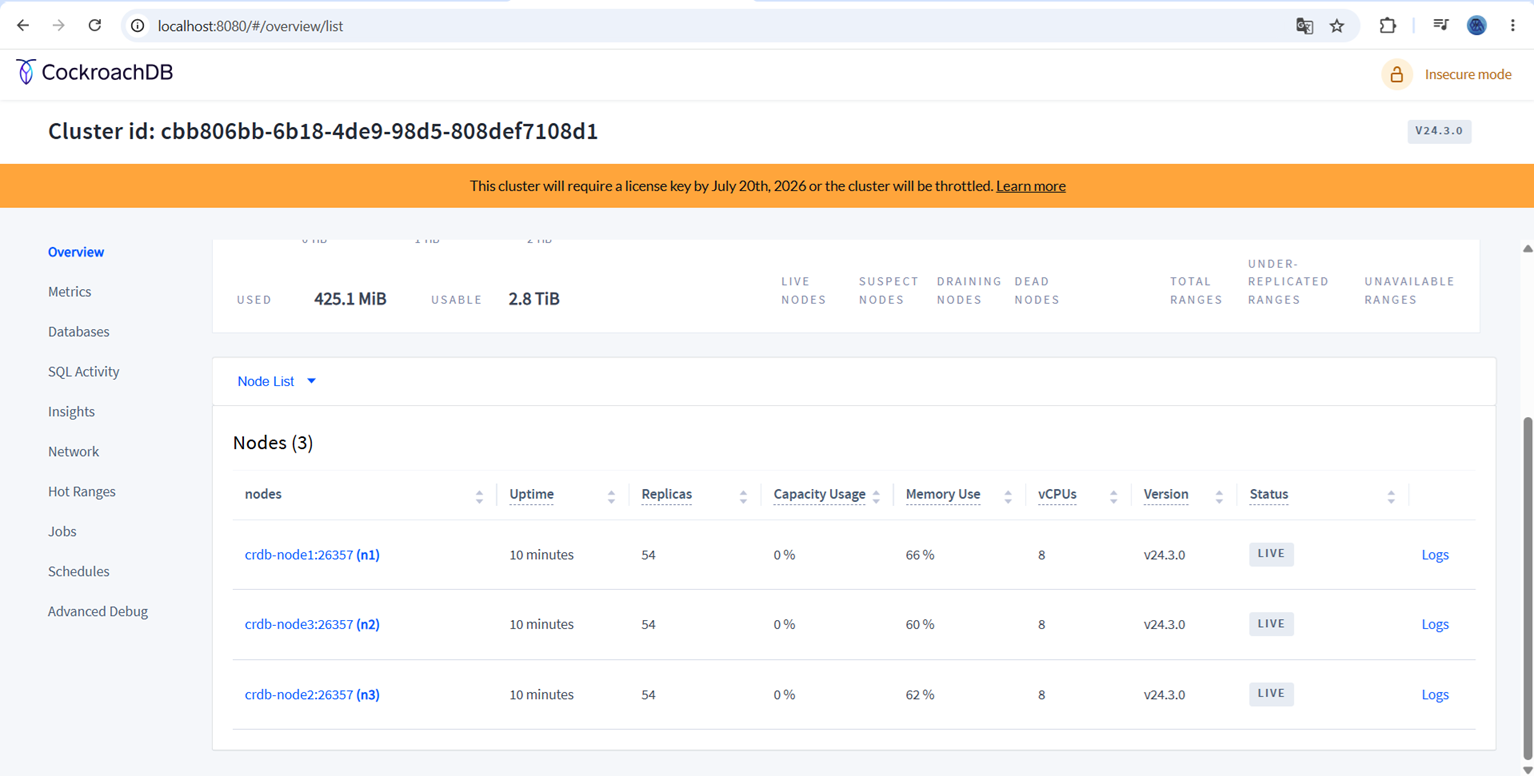
\includegraphics[width=\columnwidth]{../evidencia/dashboard.png}
\caption{Dashboard de CockroachDB (\texttt{localhost:8080}) mostrando los tres nodos activos del clúster.}
\label{fig:dashboard}
\end{figure}

\subsection{Esquema de datos de TiendaTech (Paso 2)}
El esquema (\texttt{sql/01\_schema.sql}) define cuatro tablas relacionadas: \texttt{clientes}, \texttt{productos}, \texttt{pedidos} y \texttt{detalle\_pedido}, con claves primarias, foráneas y restricciones \texttt{CHECK} de dominio. La tabla \texttt{pedidos} usa una clave primaria compuesta \texttt{(provincia\_entrega, pedido\_id)}, condición necesaria para que la fragmentación lógica por lista coincida con el prefijo de la clave primaria.

Tras crear el esquema, se aplicó la fragmentación lógica (\texttt{sql/02\_partitions.sql}): \texttt{ALTER TABLE pedidos PARTITION BY LIST (provincia\_entrega) (\ldots)}, definiendo cinco particiones. Se verificó con \texttt{SHOW PARTITIONS FROM TABLE pedidos} que las cinco particiones quedaron correctamente registradas en el catálogo (Fig. \ref{fig:particiones}).

\begin{figure}[H]
\centering
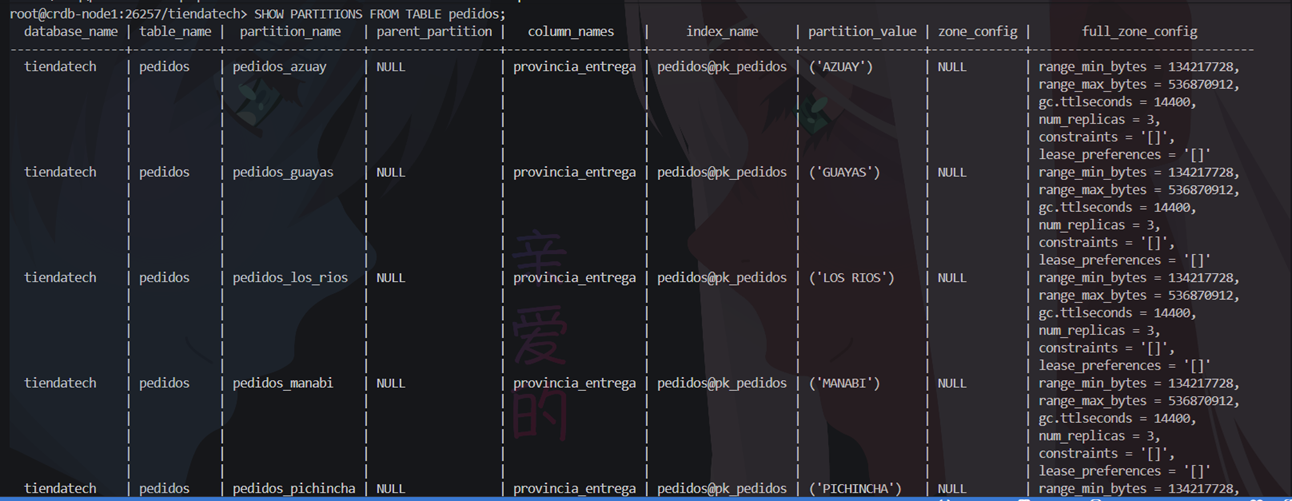
\includegraphics[width=\columnwidth]{../evidencia/particiones_pedidos.png}
\caption{Salida de \texttt{SHOW PARTITIONS FROM TABLE pedidos}: cinco particiones lógicas registradas por provincia.}
\label{fig:particiones}
\end{figure}

Se cargaron los datos con \texttt{scripts/seed\_data.py}, un script Python reproducible (semillas \texttt{random.seed(42)} y \texttt{Faker.seed(42)}) que genera y carga, mediante \texttt{psycopg2.extras.execute\_values} en lotes de 500-1000 filas: 1\,000 clientes, 500 productos, 10\,000 pedidos y 19\,884 líneas de detalle. El dataset es sintético, generado localmente con \texttt{Faker} (\textit{locale} \texttt{es\_ES}). La reproducibilidad se verificó con \texttt{SELECT COUNT(*)} sobre cada tabla (Fig. \ref{fig:carga}).

\begin{figure}[H]
\centering

\includegraphics[width=\columnwidth]{../evidencia/carga_10000_registros.png}
\caption{Confirmación de la carga de 10\,000 pedidos y 19\,884 detalles en el clúster.}
\label{fig:carga}
\end{figure}

\subsection{Composición del dataset sintético}
El generador \texttt{seed\_data.py} construye el dataset a partir de constantes explícitas: \texttt{TOTAL\_CLIENTES = 1000}, \texttt{TOTAL\_PRODUCTOS = 500}, \texttt{TOTAL\_PEDIDOS = 10\,000}. Las provincias del dominio son LOS RÍOS, GUAYAS, PICHINCHA, MANABÍ y AZUAY, asignadas mediante \texttt{random.choice}. Los productos se agrupan en seis categorías: PROCESADORES, TARJETAS GRÁFICAS, MEMORIAS RAM, ALMACENAMIENTO, PLACAS MADRE y PERIFÉRICOS. El estado de cada pedido se sortea entre PENDIENTE, PAGADO, ENVIADO, ENTREGADO y CANCELADO.

Las fechas se generan con \texttt{fecha\_inicial = datetime.now() - timedelta(days=730)} y un desplazamiento aleatorio de hasta 729 días. Cada pedido incluye entre 1 y 3 líneas de detalle, lo que explica que 10\,000 pedidos produjeran 19\,884 filas en \texttt{detalle\_pedido} —un promedio de 1.99 líneas por pedido—, cifra verificada directamente y no estimada.

\subsection{Protocolo de verificación de tolerancia a fallos (Paso 3)}
Con el clúster en operación y los 10\,000 pedidos verificados, se ejecutó el siguiente protocolo:
\begin{enumerate}[leftmargin=*]
\item Confirmar el conteo base ejecutando \texttt{SELECT COUNT(*) FROM pedidos} contra el nodo 1 (esperado: 10\,000).
\item Detener el nodo 2 con \texttt{docker stop crdb-node2}.
\item Confirmar el estado \texttt{Exited} del nodo 2 mediante \texttt{docker compose ps -a}.
\item Reejecutar \texttt{SELECT COUNT(*) FROM pedidos} contra el nodo 1, esperando el mismo resultado.
\item Esperar 30 segundos y ejecutar \texttt{SHOW RANGES FROM TABLE pedidos} para observar si existió redistribución de réplicas.
\item Reiniciar el nodo 2 con \texttt{docker start crdb-node2} y confirmar el retorno a \texttt{is\_live=true} en los tres nodos.
\end{enumerate}

\subsection{Consultas de referencia y \textit{benchmark} (Paso 4)}
Se definieron cinco consultas SQL (\texttt{sql/03\_queries.sql}): \textbf{Q1} \textit{join} \texttt{pedidos}$\Join$\texttt{clientes}; \textbf{Q2} agregación \texttt{GROUP BY} por provincia; \textbf{Q3} búsqueda puntual por clave primaria compuesta; \textbf{Q4} consulta de rango por fecha y monto; \textbf{Q5} subconsulta correlacionada de clientes con más de 5 pedidos. Cada consulta se envolvió en \texttt{EXPLAIN ANALYZE}.

El script \texttt{scripts/run\_benchmark.py} ejecuta cada consulta cinco veces (\texttt{REPETICIONES = 5}), extrae el tiempo de ejecución del plan mediante una expresión regular y calcula la media aritmética con \texttt{statistics.mean()}.

\textbf{Limitación reconocida del instrumento:} la versión del script utilizada en esta práctica descarta los cinco tiempos individuales tras calcular la media y solo persiste el promedio en \texttt{evidencia/resultados.csv}; en consecuencia, no fue posible calcular desviación estándar, mediana, mínimo, máximo ni percentiles sin inventar datos. Los resultados presentados corresponden exclusivamente a los promedios reales obtenidos durante la ejecución del \textit{benchmark}. Esta limitación se reconoce como una amenaza a la validez (Sección \ref{sec:amenazas}) y como una mejora futura del instrumento (Sección \ref{sec:trabajofuturo}).

Para la comparación distribuido vs. centralizado se creó \texttt{docker-compose-single.yml}, que despliega una única instancia CockroachDB (\texttt{crdb-single}, modo \texttt{start-single-node}) en el puerto 26260. Sobre esta instancia se replicó exactamente el mismo protocolo, garantizando que ambos entornos contienen datos idénticos y que la única variable independiente es el número de nodos.

\subsection{Registro en video de la prueba de tolerancia a fallos}
La prueba completa de tolerancia a fallos descrita en la sección anterior (pasos 1 a 6) fue registrada en video y almacenada en el repositorio del proyecto (commit \texttt{460cad0}, tag \texttt{v1.0-pe-u3}), en la siguiente ruta:
\begin{center}
\texttt{evidencia/prueba-de-tolerancia-a-fallos.mp4}
\end{center}

\subsection{Comandos de verificación utilizados}
La Tabla \ref{tab:comandos} enumera los comandos de verificación efectivamente ejecutados durante la práctica, en el orden en que se usaron.

\begin{table}[H]
\centering
\caption{Comandos de verificación ejecutados y evidencia que producen}
\label{tab:comandos}
\begin{tabularx}{\columnwidth}{p{3.6cm}X}
\toprule
\textbf{Comando} & \textbf{Propósito / evidencia}\\
\midrule
\texttt{cockroach node status} & Confirmar \texttt{is\_live=true} en los 3 nodos (Fig. \ref{fig:dashboard}, \ref{fig:reintegro}). \\
\texttt{SHOW PARTITIONS FROM TABLE pedidos;} & Verificar las 5 particiones lógicas (Fig. \ref{fig:particiones}). \\
\texttt{SELECT COUNT(*) FROM <tabla>;} & Verificar filas cargadas (Fig. \ref{fig:carga}). \\
\texttt{SHOW RANGES FROM TABLE pedidos;} & Verificar distribución física real (Fig. \ref{fig:ranges}). \\
\texttt{docker stop / start crdb-node2} & Simular y revertir la caída del nodo 2. \\
\texttt{EXPLAIN ANALYZE <consulta>;} & Obtener tiempo real y plan físico. \\
\bottomrule
\end{tabularx}
\end{table}

%==============================================================
\section{Resultados}
\label{sec:resultados}
%==============================================================

\subsection{Tolerancia a fallos}
\label{sec:tolerancia}
Antes de detener ningún nodo, \texttt{SELECT COUNT(*) FROM pedidos} devolvió \textbf{10\,000} filas contra el nodo 1 (conteo base). Tras detener el nodo 2 (\texttt{docker stop crdb-node2}) y confirmar mediante \texttt{docker compose ps -a} que su estado pasó a \texttt{Exited}, se reejecutó la misma consulta: el resultado se mantuvo en \textbf{10\,000} filas, sin error ni degradación observable.

\textbf{Explicación del quórum Raft 2/3:} CockroachDB replica cada rango en un grupo Raft de $n$ réplicas ($n=3$). Una operación solo se confirma cuando la ha reconocido un quórum de $\lceil (n+1)/2 \rceil = 2$ réplicas. Con el nodo 2 caído, el rango de \texttt{pedidos} conservó 2 de sus 3 réplicas activas (nodos 1 y 3), cantidad suficiente para alcanzar el quórum.

\textbf{Explicación de por qué SHOW RANGES no cambió tras 30 s:} existe un parámetro de configuración —\texttt{server.time\_until\_store\_dead}, con valor por defecto de 5 minutos— antes de que el clúster considere que un nodo está ``muerto'' y comience a generar réplicas de reemplazo. Dentro de la ventana de 30 segundos, el nodo 2 solo se encontraba ``sospechoso'', no ``muerto''; además, el rango seguía teniendo quórum (2/3). Por ambas razones, \texttt{SHOW RANGES} continuó reportando la misma configuración de tres réplicas $\{1,2,3\}$ (Fig. \ref{fig:ranges}).

\begin{figure}[H]
\centering
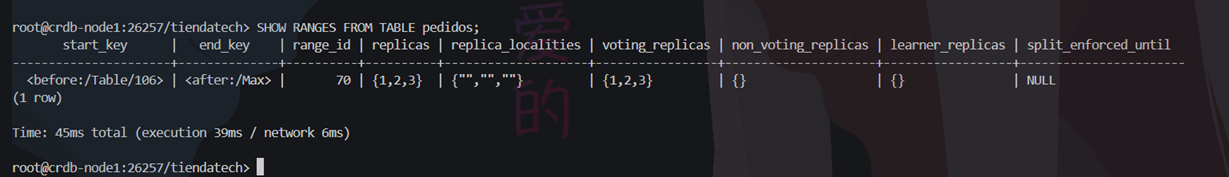
\includegraphics[width=\columnwidth]{../evidencia/show_ranges_durante_fallo.png}
\caption{Salida de \texttt{SHOW RANGES FROM TABLE pedidos} durante la caída del nodo 2: la configuración de réplicas $\{1,2,3\}$ no cambió dentro de la ventana de 30 s.}
\label{fig:ranges}
\end{figure}

La Fig. \ref{fig:raft-seq} esquematiza el comportamiento Raft observado: mientras el nodo 2 permanece caído, el cliente SQL continúa dirigiendo sus solicitudes al \textit{gateway} (nodo 1), que las enruta al líder vigente del rango; si dicho líder residía en el nodo 2, se produce una reelección resuelta entre el nodo 1 y el nodo 3.

\begin{figure*}[t]
\centering
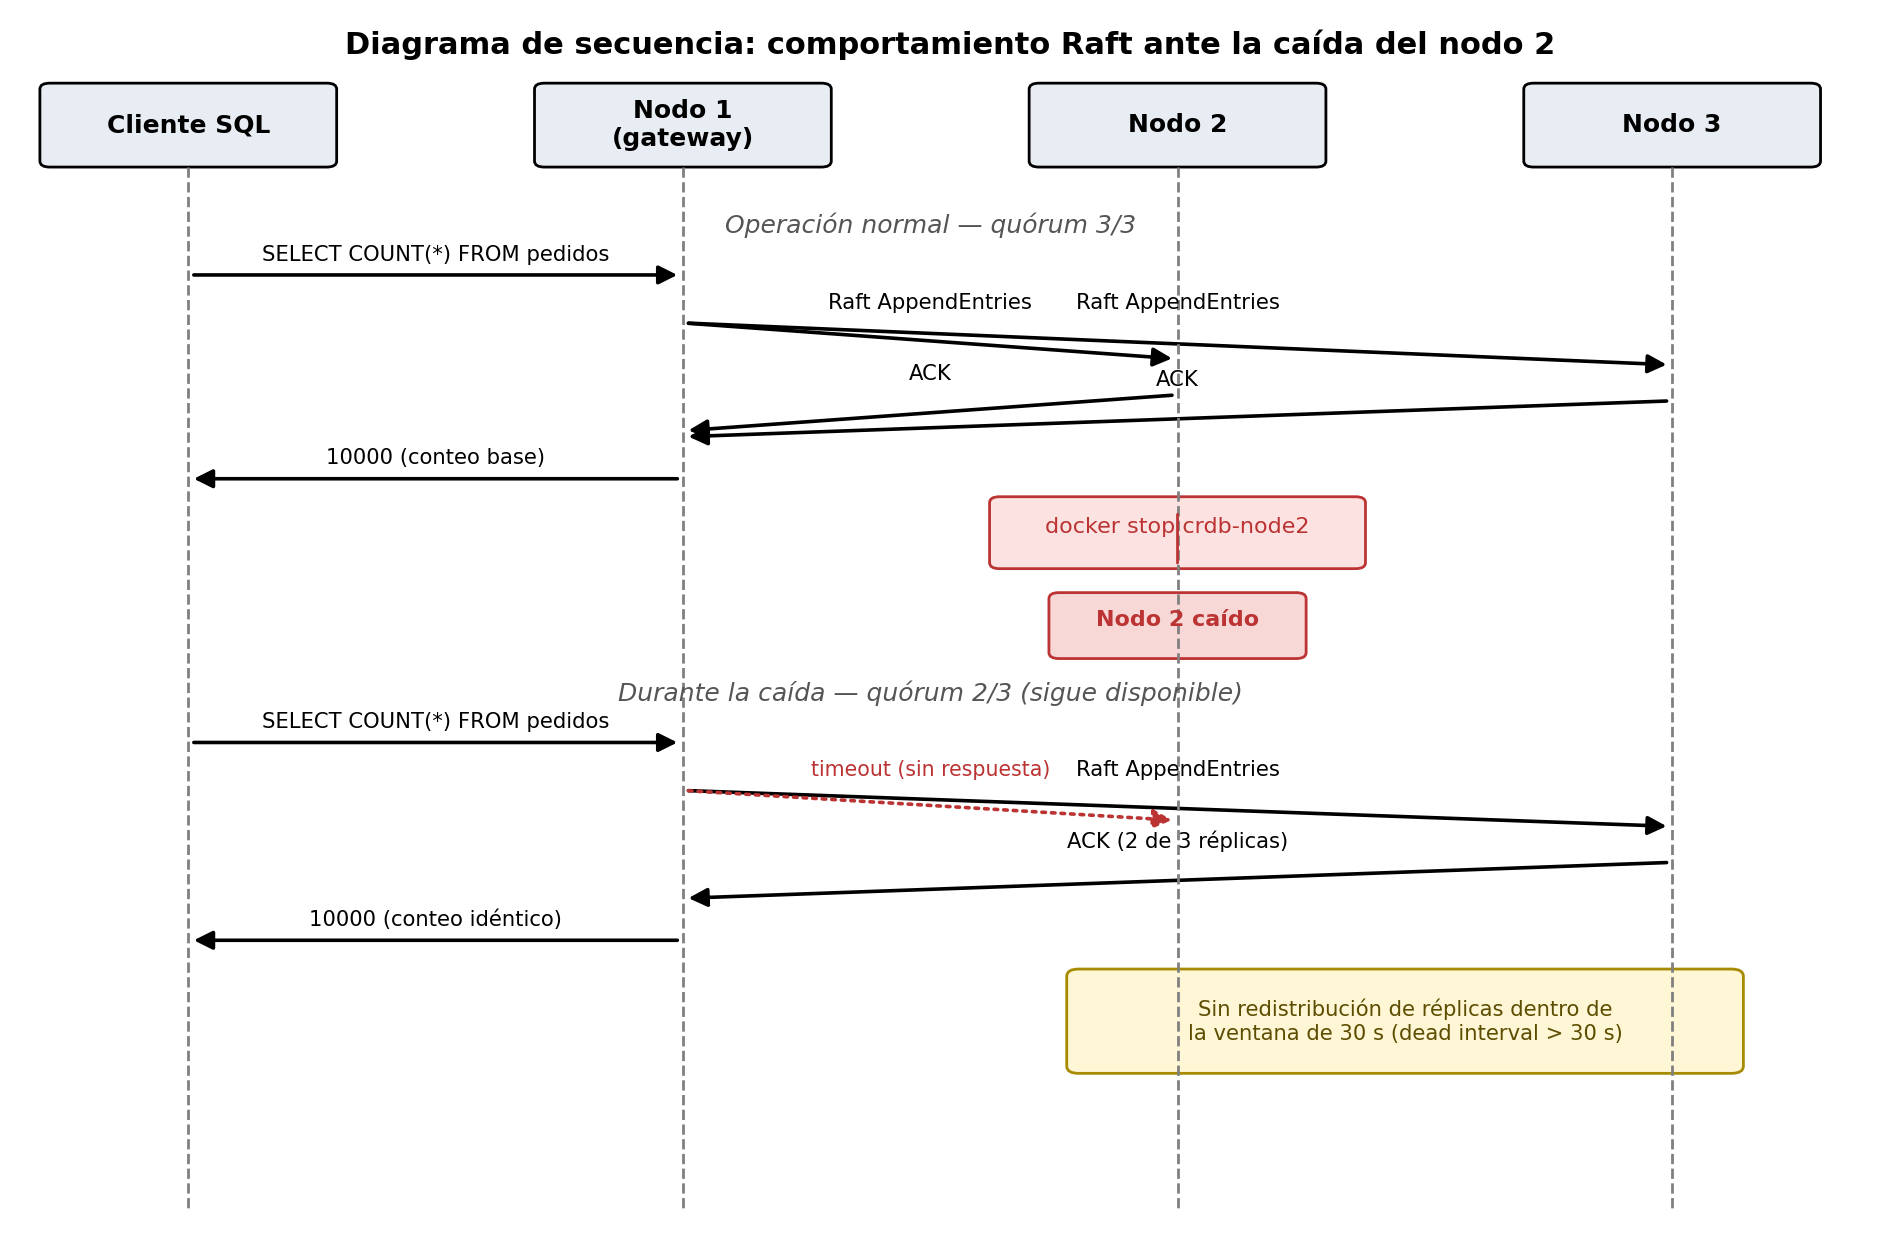
\includegraphics[width=0.85\textwidth]{../evidencia/diagrama_raft.png}
\caption{Diagrama de secuencia del comportamiento Raft ante la caída del nodo 2: el clúster mantiene disponibilidad de lectura con quórum 2/3.}
\label{fig:raft-seq}
\end{figure*}

Finalmente, se reinició el nodo 2 con \texttt{docker start crdb-node2} (Fig. \ref{fig:reintegro}). Se cronometró el tiempo de reintegración, desde la ejecución del comando hasta que \texttt{cockroach node status} reportó \texttt{is\_available=true} e \texttt{is\_live=true} en los tres nodos simultáneamente: el nodo se reintegró correctamente en \textbf{5.73 segundos}.

\begin{figure}[H]
\centering
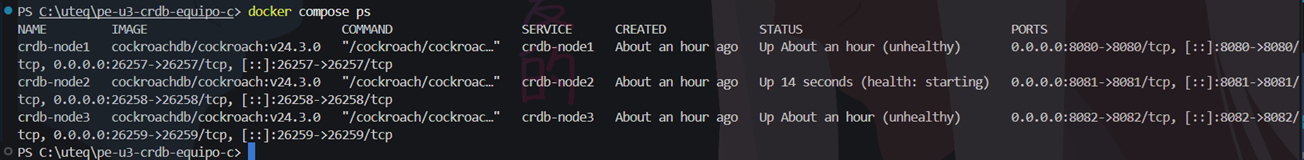
\includegraphics[width=\columnwidth]{../evidencia/nodo2_reintegrado.png}
\caption{Reintegración del nodo 2 al clúster: los tres nodos vuelven a reportar \texttt{is\_live=true} tras \texttt{docker start crdb-node2}.}
\label{fig:reintegro}
\end{figure}

\subsection{Fragmentación lógica vs. rangos físicos}
\label{sec:frag-fisica}

\textbf{Corrección respecto de una interpretación previa del equipo:} una versión anterior de este informe afirmaba que cada una de las cinco particiones lógicas de \texttt{pedidos} se almacenaba en un rango físico distinto del clúster. La evidencia recogida en la propia práctica no respalda esa afirmación.

\texttt{SHOW PARTITIONS FROM TABLE pedidos} (Fig. \ref{fig:particiones}) confirmó la existencia de cinco particiones lógicas registradas en el catálogo. Sin embargo, al ejecutar \texttt{SHOW RANGES FROM TABLE pedidos} sobre la tabla completa, el resultado devolvió \textbf{una sola fila}: un único rango cuyo \texttt{start\_key} y \texttt{end\_key} abarcan la totalidad de la tabla, con \texttt{replicas = \{1,2,3\}}.

\textbf{Interpretación técnica correcta:} \texttt{PARTITION BY LIST} crea unidades lógicas de configuración, pero no obliga a que cada partición resida en un rango físico separado. Un rango solo se subdivide cuando su tamaño supera 512 MiB o cuando se ejecuta explícitamente un comando de división. La tabla \texttt{pedidos}, con 10\,000 filas, se mantuvo muy por debajo de ese umbral: las cinco particiones lógicas coexistieron dentro de un único rango físico, replicado tres veces mediante Raft.

Esto no invalida el objetivo pedagógico de la fragmentación horizontal —la definición formal de la Sección \ref{sec:fragmentacion} y su verificación en el catálogo siguen siendo válidas—, pero sí corrige una inferencia errónea sobre la distribución física: a esta escala, la fragmentación lógica no implicó paralelismo de acceso entre rangos, y buena parte de la latencia observada corresponde a la coordinación de un único grupo Raft replicado tres veces.

\subsection{Rendimiento: clúster vs. nodo único}
La Tabla \ref{tab:resultados} presenta el tiempo promedio de ejecución (media de 5 repeticiones) de las cinco consultas, junto con el factor de comparación $F = t_{\text{nodo único}} / t_{\text{clúster}}$: $F<1$ favorece al nodo único y $F>1$ favorece al clúster.

\begin{table}[H]
\centering
\caption{Tiempo promedio de ejecución (ms, $n=5$) y factor de comparación entre nodo único y clúster}
\label{tab:resultados}
\begin{tabularx}{\columnwidth}{Xrrrl}
\toprule
{\small\textbf{Consulta}} & {\small\textbf{Clúst.}} & {\small\textbf{N.ú.}} & {\small\textbf{$F$}} & {\small\textbf{Mejor}}\\
\midrule
{\small Q1 -- \textit{Join}}          & {\small 6.8}  & {\small 5.4}  & {\small 0.794} & {\small N. único}\\
{\small Q2 -- \texttt{GROUP BY}}      & {\small 12.2} & {\small 12.0} & {\small 0.984} & {\small N. único}\\
{\small Q3 -- Clave primaria}         & {\small 1.4}  & {\small 0.449}& {\small 0.321} & {\small N. único}\\
{\small Q4 -- Rango}                  & {\small 12.8} & {\small 14.4} & {\small 1.125} & {\small Clúster}\\
{\small Q5 -- Subconsulta}            & {\small 15.0} & {\small 22.8} & {\small 1.520} & {\small Clúster}\\
\bottomrule
\end{tabularx}
\end{table}

Los resultados fueron \textbf{mixtos}: el nodo único presentó menor tiempo promedio en Q1, Q2 y Q3, mientras que el clúster fue más rápido en Q4 y Q5. Por tanto, no se puede afirmar que uno de los dos entornos superó al otro en todas las consultas; el rendimiento relativo dependió del tipo y del costo de procesamiento de cada operación.

\begin{figure}[H]
\centering
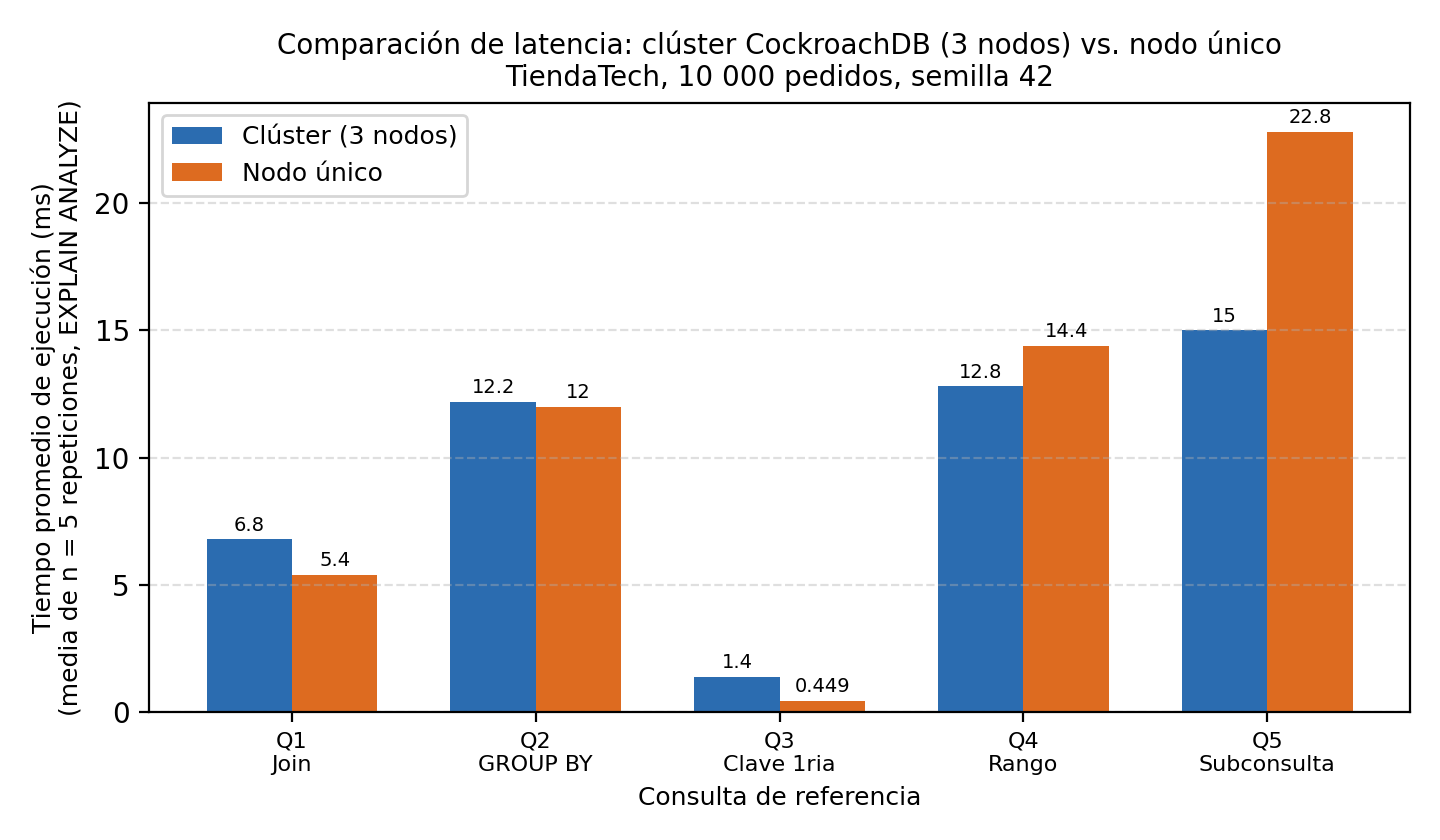
\includegraphics[width=\columnwidth]{../evidencia/grafico_comparativo.png}
\caption{Gráfico comparativo de la latencia promedio (ms) por consulta, clúster de 3 nodos vs. nodo único, generado a partir de \texttt{evidencia/resultados.csv}.}
\label{fig:comparacion}
\end{figure}

\textbf{Nota sobre reproducibilidad del gráfico:} el gráfico anterior se generó con un script Python (\texttt{matplotlib}) que lee directamente los cinco pares de valores promedio de \texttt{evidencia/resultados.csv}; no contiene valores estimados ni inventados.

\subsection{Análisis del plan de ejecución (EXPLAIN ANALYZE)}
Más allá del tiempo total, el plan físico capturado por \texttt{EXPLAIN ANALYZE} explica por qué algunas consultas se comportaron distinto. La Fig. \ref{fig:planq1} muestra el plan real de Q1 en el clúster: el optimizador eligió un \textbf{\textit{lookup join}} —para cada fila de \texttt{pedidos} escaneada, se realiza una búsqueda puntual contra \texttt{clientes@clientes\_pkey}—, con un tiempo acumulado en KV de 24 ms y un uso máximo de memoria de 240 KiB.

\begin{figure}[H]
\centering

\includegraphics[width=\columnwidth]{../evidencia/explain_analyze_cluster.png}
\caption{Plan de ejecución real de Q1 (\texttt{EXPLAIN ANALYZE}) en el clúster: \textit{lookup join} entre \texttt{pedidos} y \texttt{clientes}.}
\label{fig:planq1}
\end{figure}

\textbf{Interpretación:} un \textit{lookup join} emite, por cada fila del lado externo, una solicitud KV independiente hacia el nodo que posee la réplica líder de \texttt{clientes}; en un nodo único esas solicitudes se resuelven en memoria local, mientras que en el clúster cada una implica, en el peor caso, una llamada gRPC entre nodos, lo que explica una parte relevante de los 6.8 ms de Q1 en el clúster frente a los 5.4 ms del nodo único.

La Fig. \ref{fig:planq3} muestra el plan de Q3, donde el optimizador reportó \textbf{\texttt{actual row count: 1}}, confirmando un acceso directo por índice. Aun así, Q3 fue la consulta donde el nodo único obtuvo mayor ventaja relativa (factor 0.321): al tratarse de la operación de menor costo computacional posible, el tiempo total en el clúster quedó dominado casi por completo por el costo fijo de coordinación Raft. Este mismo razonamiento no se sostiene, sin embargo, para Q4 y Q5, donde el clúster fue más rápido; la Sección \ref{sec:sintesis} profundiza en esta aparente contradicción.

\begin{figure}[H]
\centering

\includegraphics[width=\columnwidth]{../evidencia/explain_consulta_clave_primaria.png}
\caption{Plan de ejecución real de Q3 (\texttt{EXPLAIN ANALYZE}): búsqueda puntual por clave primaria compuesta, \texttt{actual row count = 1}.}
\label{fig:planq3}
\end{figure}

\subsection{Síntesis cuantitativa de resultados}
\label{sec:sintesis}
Se calcula el promedio simple de los cinco factores $F$: $(0.794 + 0.984 + 0.321 + 1.125 + 1.520)/5 = \mathbf{0.949}$. Este resultado, cercano a 1, indica un rendimiento global similar entre ambos entornos, aunque oculta diferencias importantes entre consultas: el nodo único fue más rápido en tres de las cinco consultas (Q1, Q2, Q3), mientras que el clúster obtuvo mejores resultados en las otras dos (Q4, Q5).

La mayor ventaja del nodo único ocurrió en Q3, donde fue aproximadamente \textbf{3.12 veces más rápido} ($1/0.321$). La mayor ventaja del clúster ocurrió en Q5, donde fue \textbf{1.52 veces más rápido}. En Q2, ambos entornos presentaron tiempos prácticamente equivalentes (12.2 ms vs. 12.0 ms). Por tanto, no existió un ganador uniforme: el rendimiento dependió del tipo de consulta y de su costo de procesamiento.

%==============================================================
\section{Discusión}
\label{sec:discusion}
%==============================================================

\subsection{Contraste con trabajos relacionados}
Los resultados de rendimiento se contrastan con cuatro trabajos académicos indexados, separando lo que reportan de la interpretación que se hace de ellos.

\textbf{(a) Taft et al. (2020).} Los autores documentan que CockroachDB prioriza deliberadamente la consistencia serializable y la tolerancia a fallos sobre la latencia mínima de una única instancia \citep{taft2020cockroachdb}. \textit{Interpretación:} nuestros datos son parcialmente coherentes: en las consultas de menor costo (Q1-Q3) el sobrecosto de coordinación fue visible, pero en Q4-Q5 el clúster fue más rápido, lo que sugiere que el costo de la replicación síncrona no domina cuando el procesamiento es suficientemente pesado.

\textbf{(b) Pina, Sá y Bernardino (2023).} Los autores reportan que CockroachDB fue, de tres bases NewSQL evaluadas, la de mayores latencias, aunque con mejor escalabilidad \citep{pina2023newsql}. \textit{Interpretación:} nuestros resultados coincidieron parcialmente con este estudio. El nodo único fue más rápido en Q1, Q2 y Q3; sin embargo, el clúster obtuvo menores tiempos en Q4 y Q5. Esto indica que, con 10\,000 pedidos, el costo de coordinación distribuida afectó principalmente a las consultas simples, mientras que las consultas de mayor procesamiento pudieron beneficiarse del entorno distribuido.

\textbf{(c) Li, Liu y Li (2022).} Identifican que el diseño de líder fuerte de Raft se convierte en cuello de botella cuando crece la concurrencia \citep{li2022raft}. \textit{Interpretación:} aunque nuestro \textit{benchmark} no generó concurrencia, el mecanismo que describen es consistente con la penalización observada en Q3 (nodo único 3.12$\times$ más rápido), pero no explica por qué el clúster superó al nodo único en Q4 y Q5.

\textbf{(d) Assad, Meiklejohn, Miller y Krusche (2024).} Describen una herramienta de inyección de fallos que soporta explícitamente CockroachDB \citep{assad2024fault}. \textit{Interpretación:} nuestra prueba de tolerancia a fallos usó un método manual equivalente (\texttt{docker stop}) pero limitado a un único escenario; la Sección \ref{sec:trabajofuturo} retoma este trabajo.

\textbf{Síntesis:} los trabajos analizados explican el costo de coordinación, replicación y liderazgo de Raft en CockroachDB. Los resultados de esta práctica fueron mixtos: el nodo único presentó mejor rendimiento en tres consultas, mientras que el clúster fue más rápido en dos. La sobrecarga distribuida no afectó de manera uniforme a todas las operaciones, sino que dependió del tipo y costo de cada consulta.

\subsection{Amenazas a la validez}
\label{sec:amenazas}
\begin{enumerate}[leftmargin=*]
\item \textbf{Validez interna — entorno compartido de recursos:} ambos entornos se ejecutaron en la misma máquina host, compitiendo por CPU y E/S de disco.
\item \textbf{Validez interna — ausencia de calentamiento y de estadística por repetición:} el script solo conservó el promedio, no la dispersión entre repeticiones.
\item \textbf{Validez externa — escala del dataset:} 10\,000 pedidos es un volumen reducido; los resultados mixtos no deben extrapolarse a escenarios de millones de filas.
\item \textbf{Validez externa — ausencia de concurrencia:} no se evaluó el comportamiento bajo múltiples conexiones concurrentes.
\item \textbf{Validez de constructo:} el tiempo de \texttt{EXPLAIN ANALYZE} excluye la latencia de red entre la aplicación Python y el clúster.
\end{enumerate}

\subsection{Trabajo futuro}
\label{sec:trabajofuturo}
\begin{enumerate}[leftmargin=*]
\item \textbf{Instrumentar el benchmark para conservar datos crudos por repetición}, permitiendo calcular desviación estándar, mediana y percentiles.
\item \textbf{Adoptar una herramienta de inyección de fallos automatizada} \citep{assad2024fault}, ampliando la prueba más allá de la caída de un nodo completo.
\item \textbf{Repetir el benchmark a mayor escala y con concurrencia}, para verificar si la proporción de consultas favorables al clúster aumenta con el volumen \citep{pina2023newsql}, y forzar la división en múltiples rangos físicos.
\item \textbf{Medir la latencia end-to-end percibida por el cliente}, complementando \texttt{EXPLAIN ANALYZE} con mediciones del lado de la aplicación.
\end{enumerate}

%==============================================================
\section{Conclusiones}
\label{sec:conclusiones}
%==============================================================
\textbf{RQ1.} Se desplegó un clúster CockroachDB v24.3.0 de tres nodos en contenedores Docker, y se implementó el esquema de cuatro tablas de TiendaTech con fragmentación lógica \texttt{PARTITION BY LIST} en cinco particiones, verificadas mediante \texttt{SHOW PARTITIONS}. Se cargaron 10\,000 pedidos y 19\,884 detalles de forma reproducible (semilla 42).

\textbf{RQ2.} El clúster preservó la disponibilidad y la consistencia de lectura durante la caída del nodo 2. La consulta \texttt{SELECT COUNT(*) FROM pedidos} devolvió 10\,000 registros antes y después de detener el nodo, sin presentar errores, confirmando el quórum Raft de 2 de 3 réplicas. Tras \texttt{docker start crdb-node2}, el nodo se reintegró correctamente en un tiempo medido de \textbf{5.73 segundos}.

\textbf{RQ3.} Los resultados de rendimiento fueron mixtos. El nodo único presentó menor tiempo promedio en Q1, Q2 y Q3, mientras que el clúster fue más rápido en Q4 y Q5. La mayor ventaja del nodo único ocurrió en Q3 (3.12$\times$); la mayor ventaja del clúster ocurrió en Q5 (1.52$\times$). El promedio de los cinco factores fue \textbf{0.949}, cercano a 1, indicando un rendimiento global semejante, aunque este promedio no representó por completo las diferencias individuales.

La tabla \texttt{pedidos} permaneció en un único rango físico replicado en los tres nodos; por tanto, las diferencias de rendimiento no estuvieron relacionadas con la distribución entre varios rangos físicos, sino con el procesamiento de cada consulta y la coordinación distribuida realizada por CockroachDB.

Se concluyó que el principal beneficio del clúster para TiendaTech fue la continuidad del servicio ante la caída de un nodo. No se encontró un entorno uniformemente más rápido para todas las consultas, por lo que la selección entre un clúster y un nodo único debe considerar tanto la disponibilidad requerida como los patrones reales de acceso del sistema.

%==============================================================
\section{Anexos}
%==============================================================

\subsection*{A.1 Consistencia de CockroachDB ante fallo de nodo (algoritmo Raft)}
CockroachDB divide cada tabla en rangos y replica cada rango en un grupo Raft independiente —en la práctica realizada, la tabla \texttt{pedidos} completa correspondió a un único rango (Sección \ref{sec:frag-fisica})—. Una réplica es elegida líder mediante elecciones basadas en \textit{heartbeats}; una entrada del \textit{log} se considera comprometida solo cuando la ha persistido un quórum de $\lceil (n+1)/2 \rceil$ réplicas. Si el líder falla, los seguidores restantes detectan la ausencia de \textit{heartbeats} y convocan una nueva elección.

\subsection*{A.2 CockroachDB (Serializable) vs. Apache Cassandra (consistencia eventual)}
\label{sec:anexoA2}
CockroachDB ofrece \texttt{SERIALIZABLE}; Cassandra ofrece consistencia ajustable por cuórum (\texttt{ONE}, \texttt{QUORUM}, \texttt{ALL}). Para TiendaTech, cuyo dominio exige integridad referencial estricta, se elegiría CockroachDB: perder consistencia en una venta tiene mayor costo de negocio que la penalización de latencia medida en esta práctica.

\subsection*{A.3 Fragmentación horizontal explícita con PARTITION BY RANGE}
Una estrategia complementaria a \texttt{LIST} sería \texttt{PARTITION BY RANGE} sobre \texttt{fecha\_pedido}. Al igual que con la partición por lista, definir particiones lógicas por rango de fecha no garantizaría por sí sola una distribución física en múltiples rangos si el volumen total permanece bajo 512 MiB.

\subsection*{A.4 Atomicidad multi-tabla en distintos nodos: 2PC interno}
CockroachDB garantiza atomicidad mediante una variante interna del compromiso en dos fases: el nodo \textit{gateway} designa un registro de transacción y coordina un \texttt{Prepare} implícito escribiendo valores \textit{intent}; solo cuando todos se han escrito exitosamente se marca la transacción como \texttt{COMMITTED}.

\subsection*{A.5 Preguntas de reflexión adicionales}
A 10\,000\,000 de pedidos, la tabla superaría el umbral de 512 MiB, forzando su división en decenas de rangos; en ese escenario, la fragmentación lógica por provincia sí podría traducirse en rangos físicos diferenciados si se combina con una directiva explícita de pre-división (\texttt{ALTER TABLE ... SPLIT AT}).

%==============================================================
\bibliographystyle{unsrt}
\bibliography{referencias}

\end{document}
